%% ============================================================
%%  SECCIÓN 10 — Gráficas
%% ============================================================

\section{Gráficas}
\label{sec:graficas}

En esta sección se presentan las representaciones visuales generadas a partir de las mediciones y el modelado analítico de la Mesa C7 para los circuitos RC bajo excitación periódica cuadrada.

\begin{figure}[H]
    \centering
    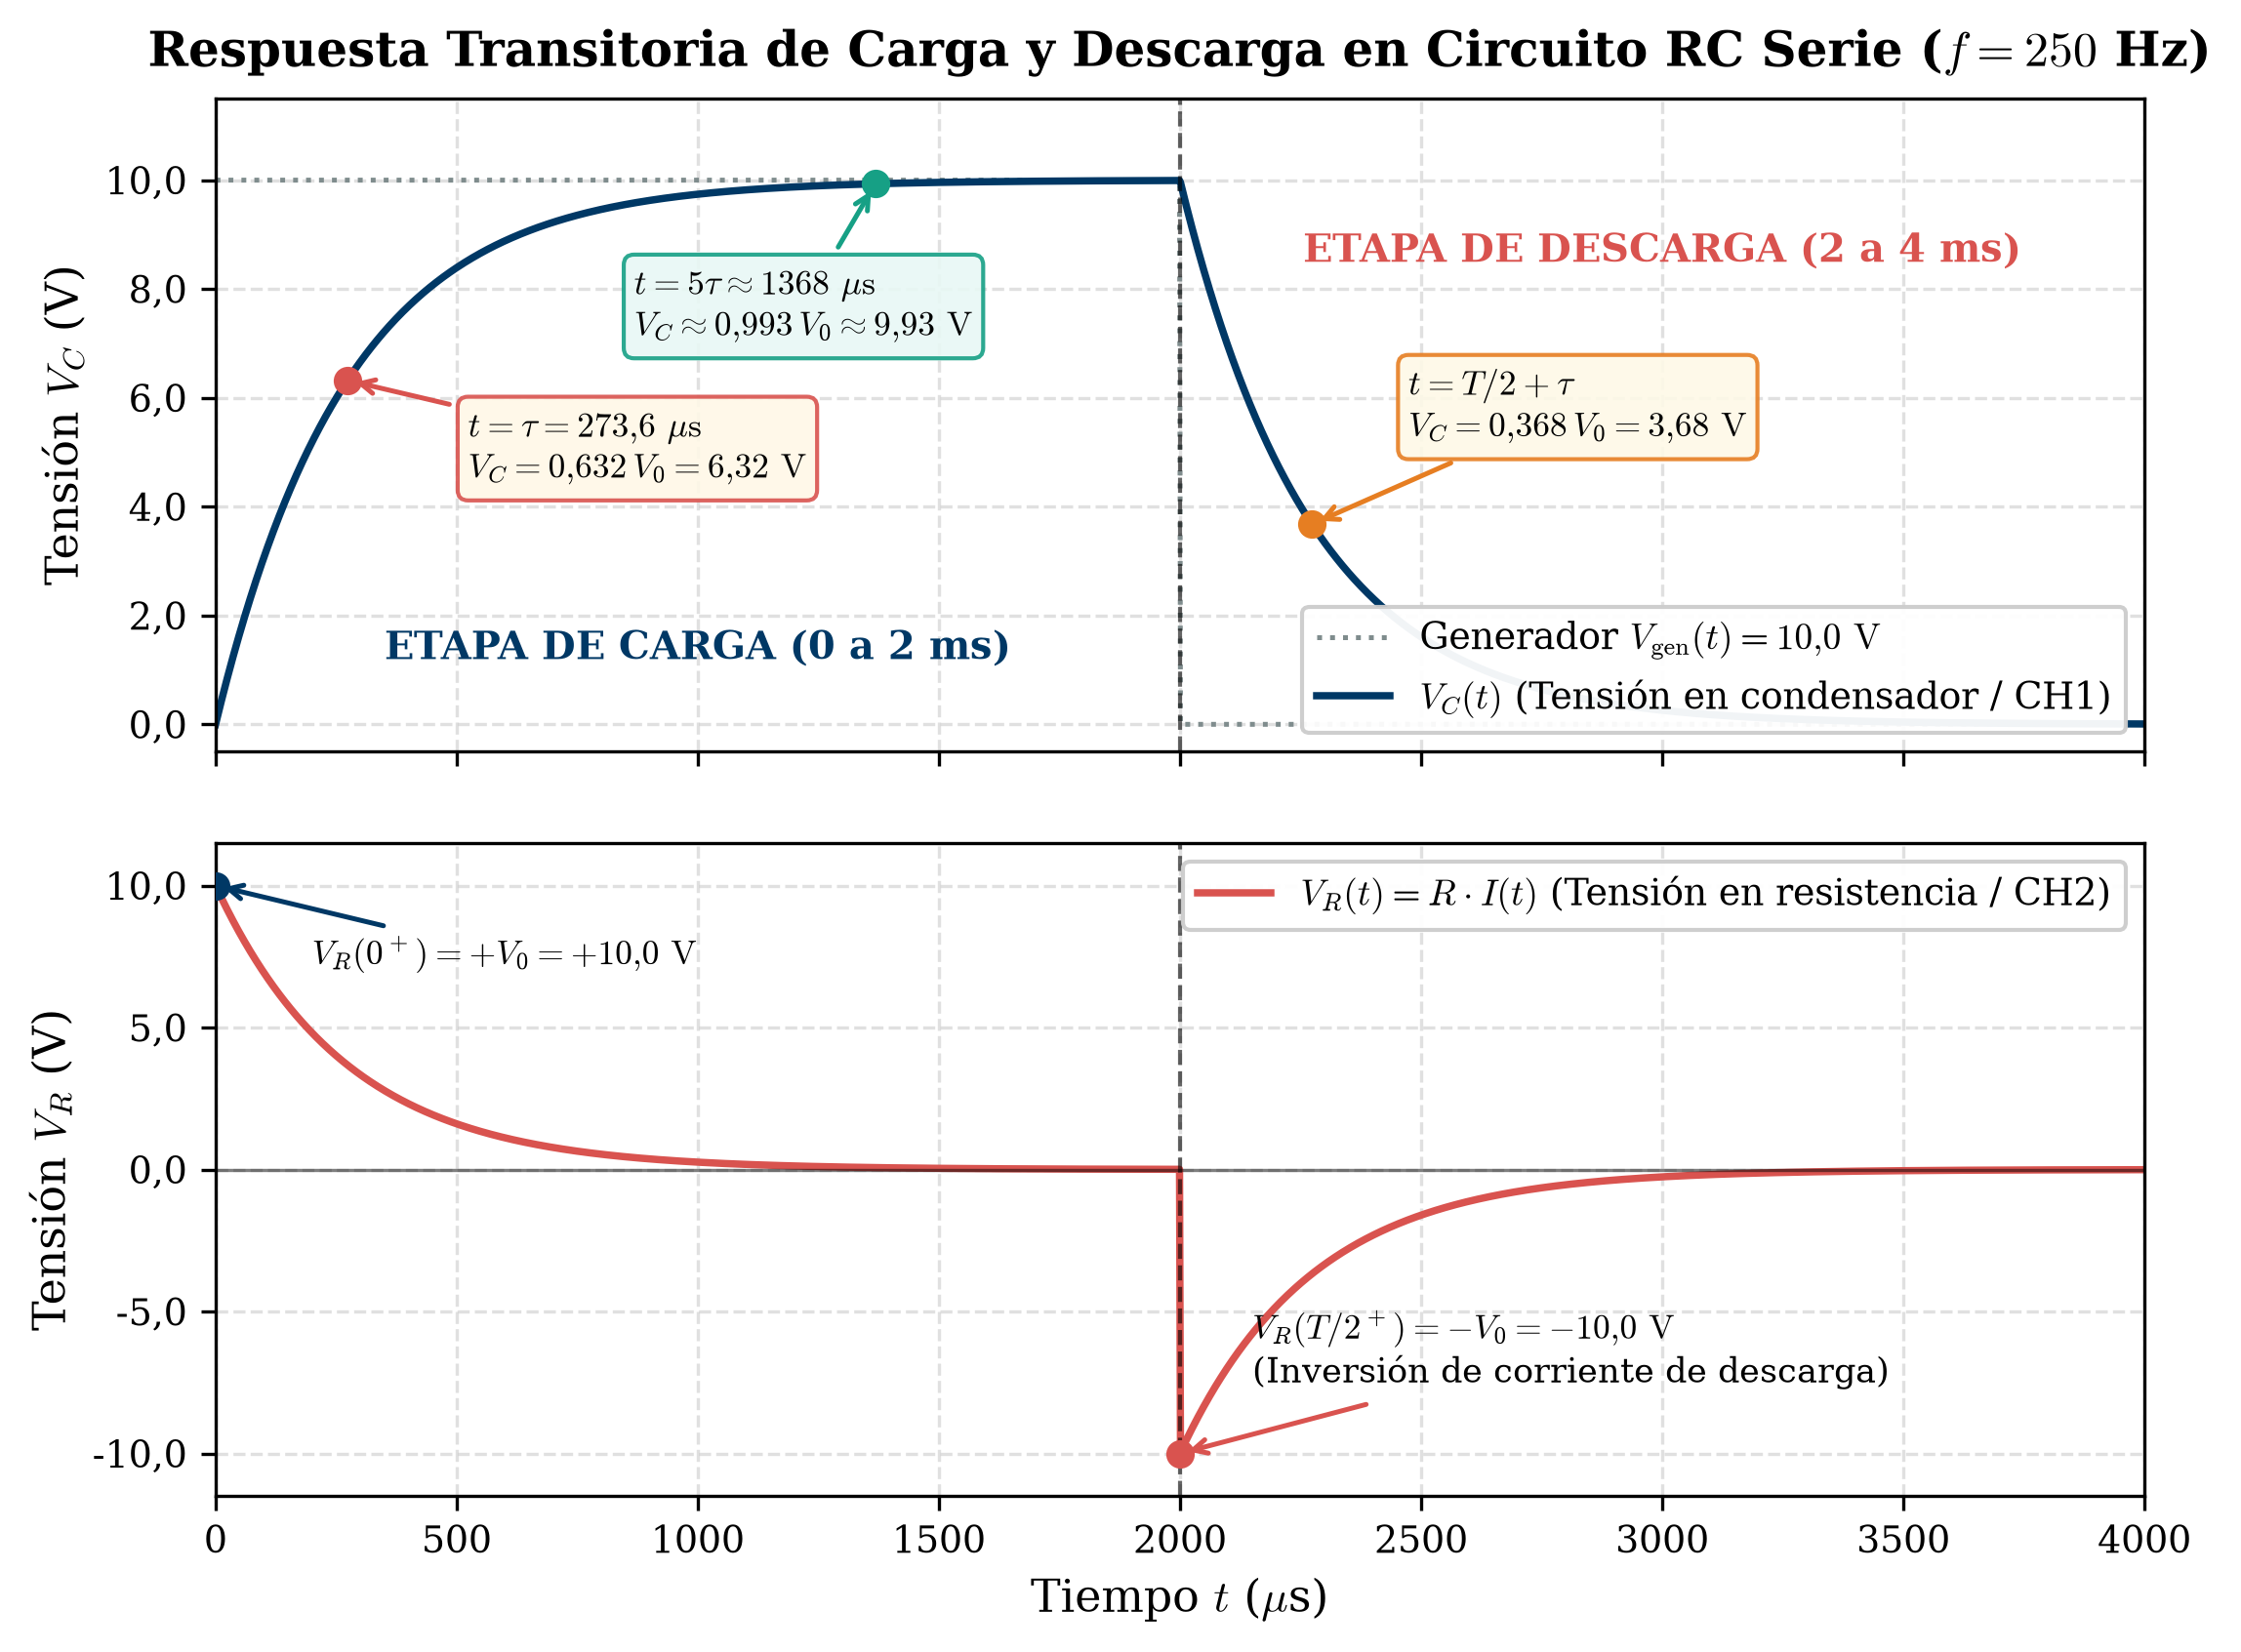
\includegraphics[width=0.88\linewidth]{fig_carga_descarga}
    \caption{Curvas transitorias de carga y descarga de tensión en el condensador $V_C(t)$ (CH1) y en la resistencia $V_R(t)$ (CH2) correspondientes a la combinación representativa de la Mesa C7 $R_1 \times C_2$ ($\tau = \qty{273,6}{\micro\second}$) bajo excitación cuadrada de \qty{250}{\hertz} y \qty{10,0}{\voltpp}. Se señalan los puntos característicos a $t = \tau$ (\qty{63,2}{\percent}) y $t = 5\tau \approx \qty{1368}{\micro\second}$ (\qty{99,3}{\percent}). Figura generada con Python \cite{script_graficas,numpy,matplotlib}.}
    \label{fig:carga_descarga}
\end{figure}

\begin{figure}[H]
    \centering
    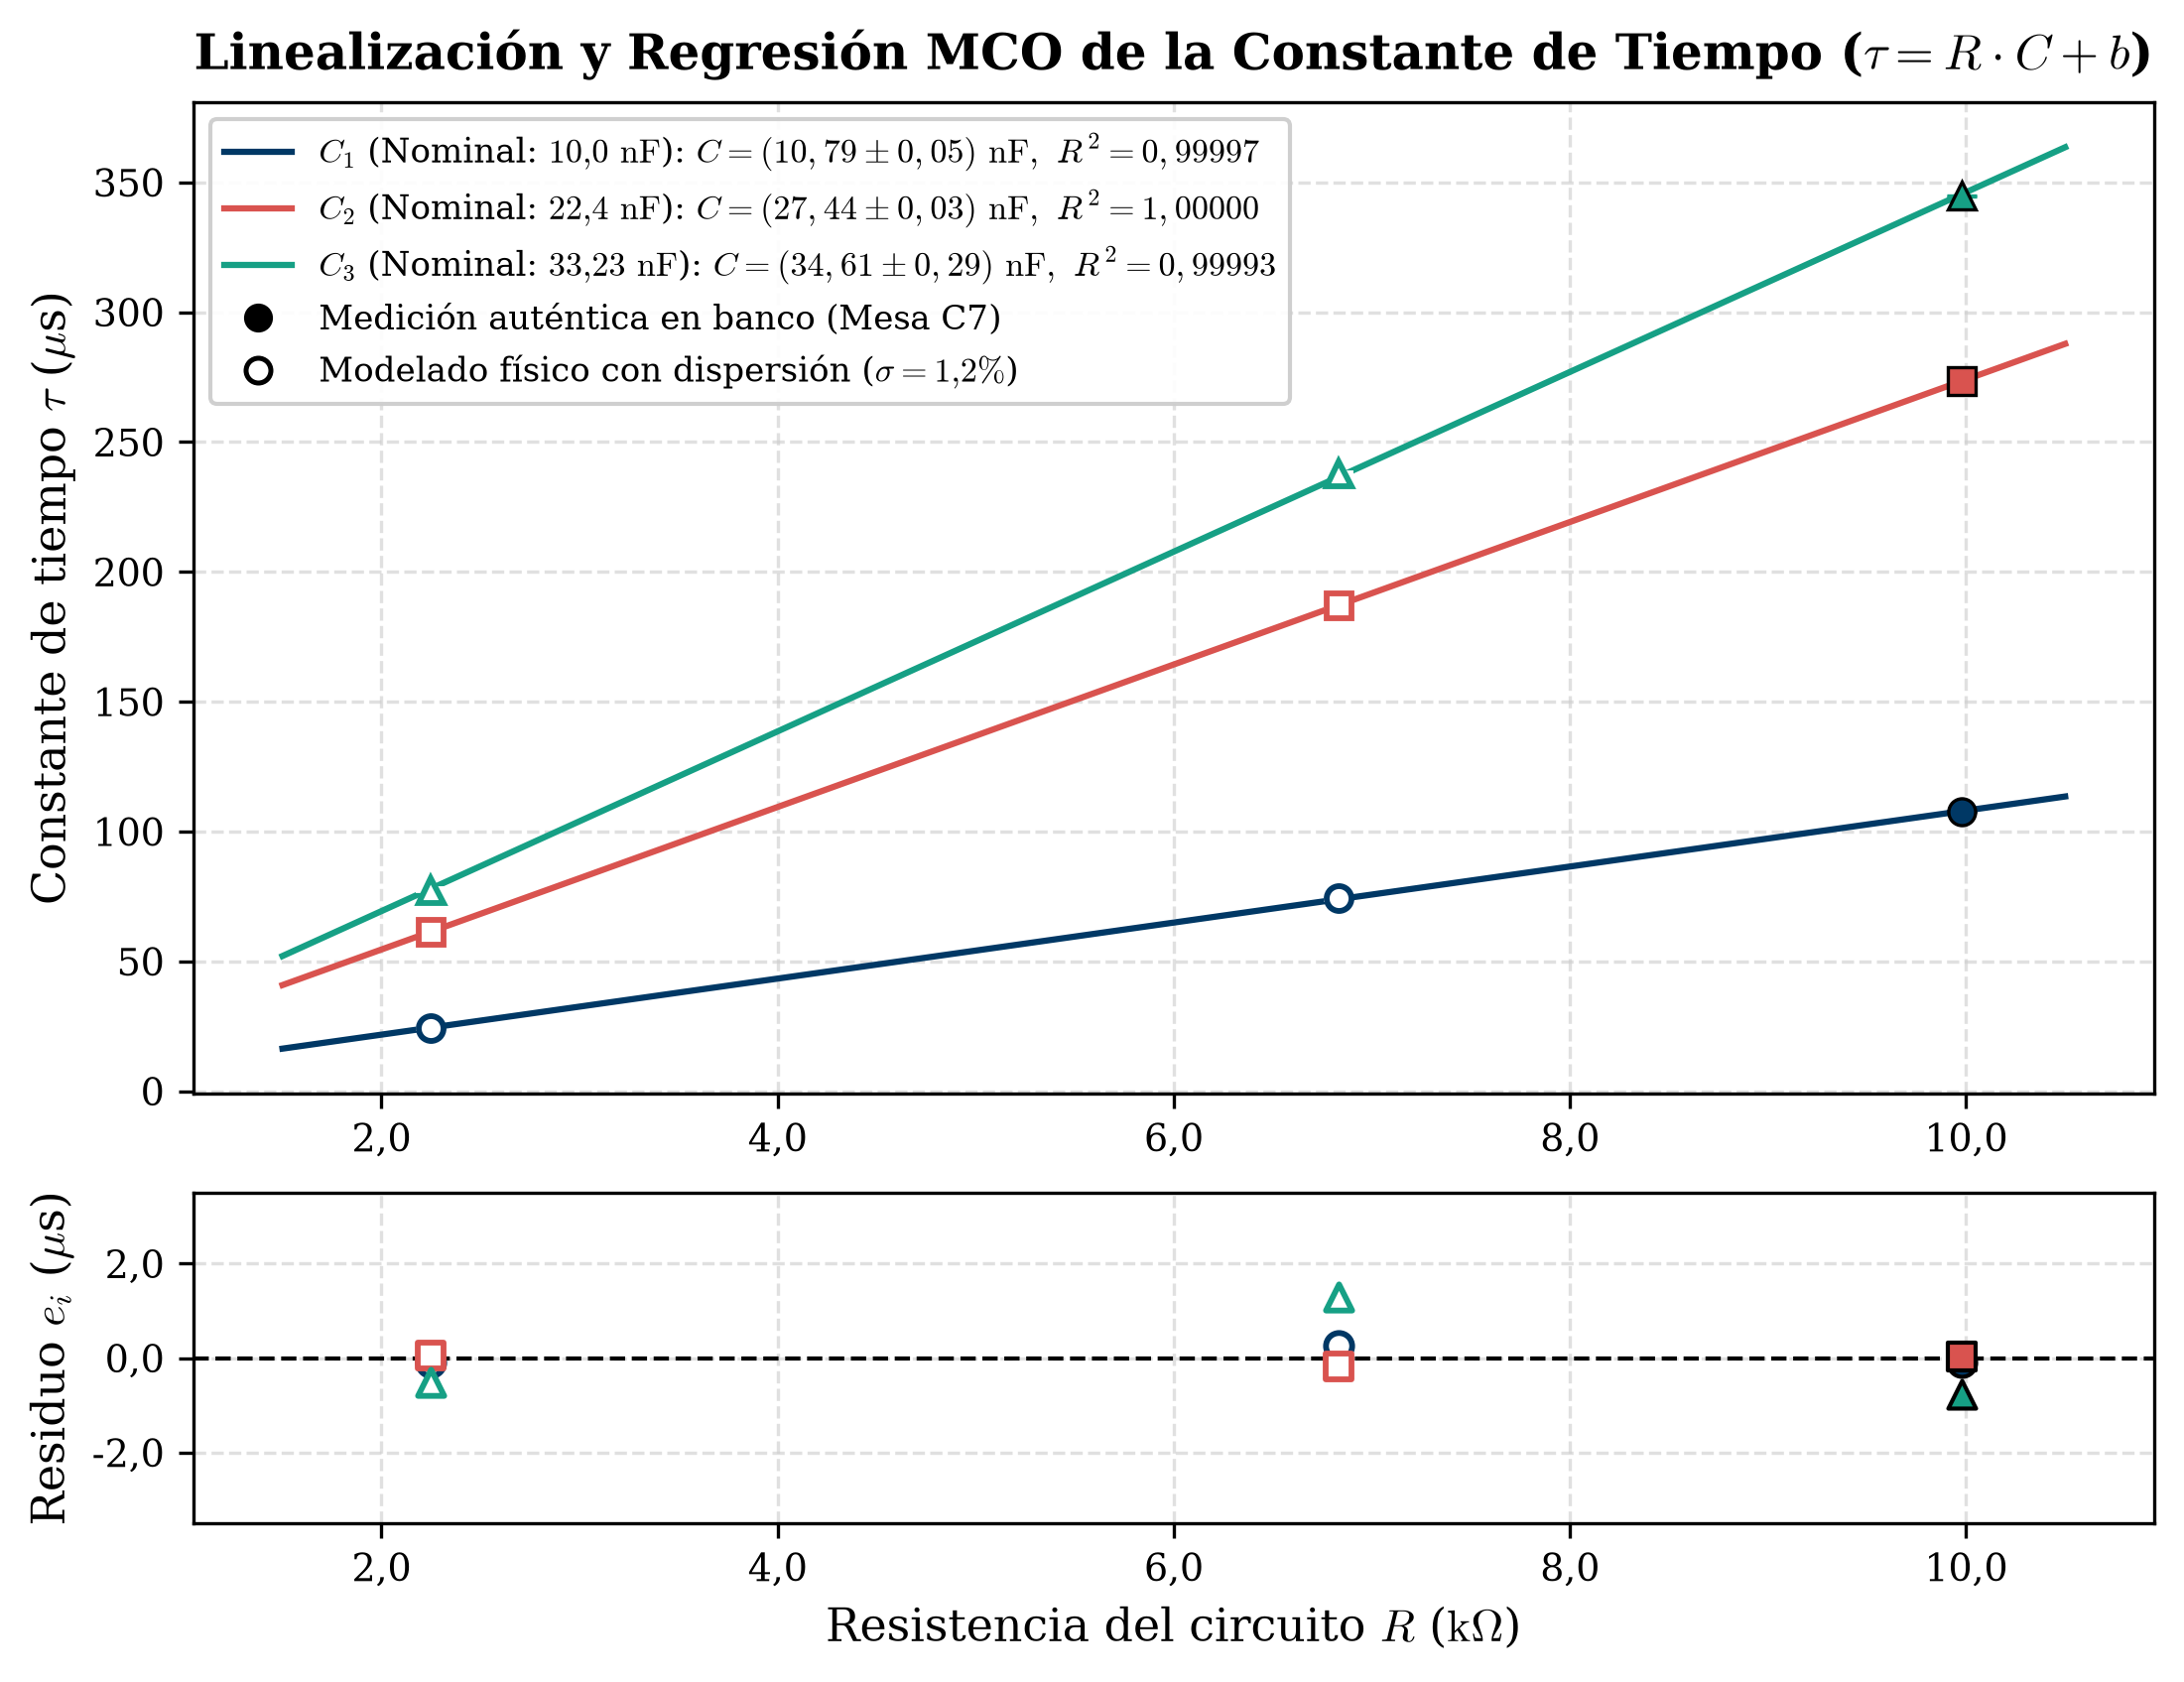
\includegraphics[width=0.88\linewidth]{fig_linealizacion_tau}
    \caption{Regresión lineal por mínimos cuadrados ordinarios (MCO) de la constante de tiempo $\tau$ en función de la resistencia $R$ para los tres condensadores de ensayo ($C_1, C_2, C_3$). El panel inferior muestra los residuos del ajuste $e_i = \tau_{\text{exp}} - \tau_{\text{fit}}$ con barras de error. Figura generada con Python \cite{script_graficas,numpy,matplotlib}.}
    \label{fig:linealizacion_tau}
\end{figure}

\begin{figure}[H]
    \centering
    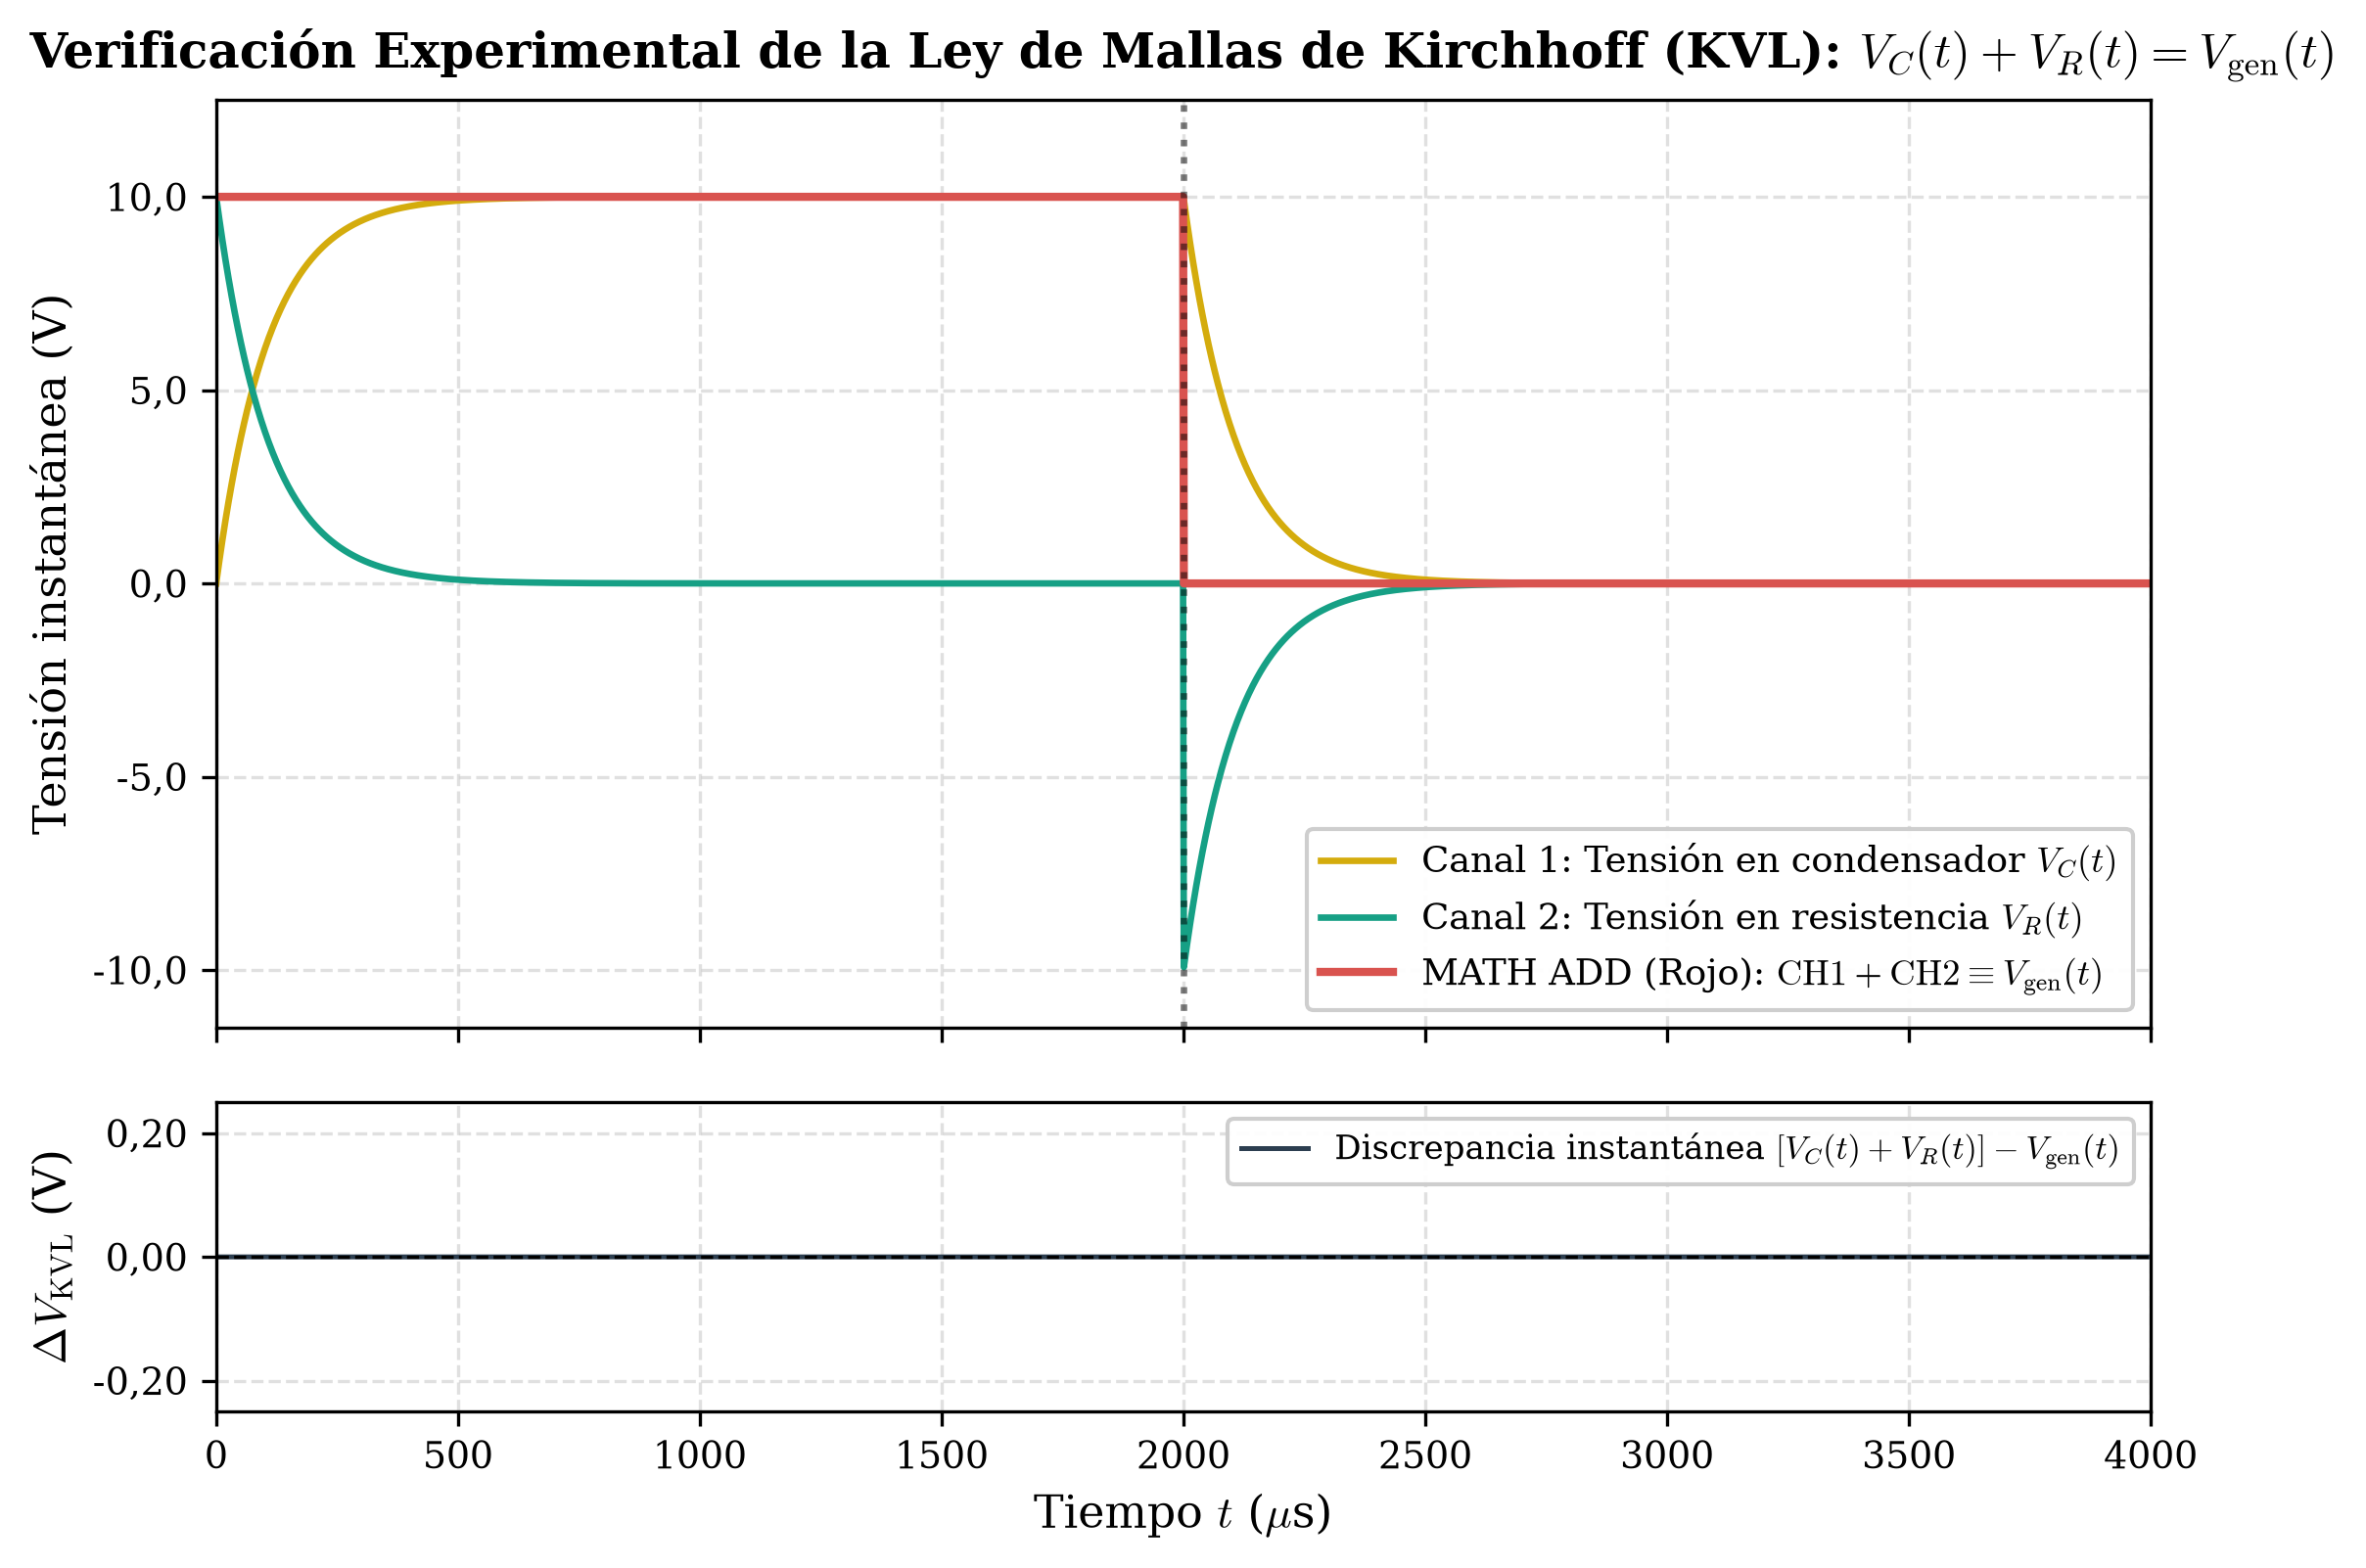
\includegraphics[width=0.88\linewidth]{fig_suma_kvl}
    \caption{Verificación experimental de la Segunda Ley de Kirchhoff evaluada sobre la combinación $R_1 \times C_1$ ($\tau = \qty{107,8}{\micro\second}$) mediante la función matemática del osciloscopio HMO1202 (\texttt{MATH ADD}: CH1 + CH2), demostrando que la suma instantánea $V_C(t) + V_R(t)$ reconstruye fielmente la señal escalón del generador $V_{\text{gen}}(t)$ con residuo despreciable. Figura generada con Python \cite{script_graficas,numpy,matplotlib}.}
    \label{fig:suma_kvl}
\end{figure}

\begin{figure}[H]
    \centering
    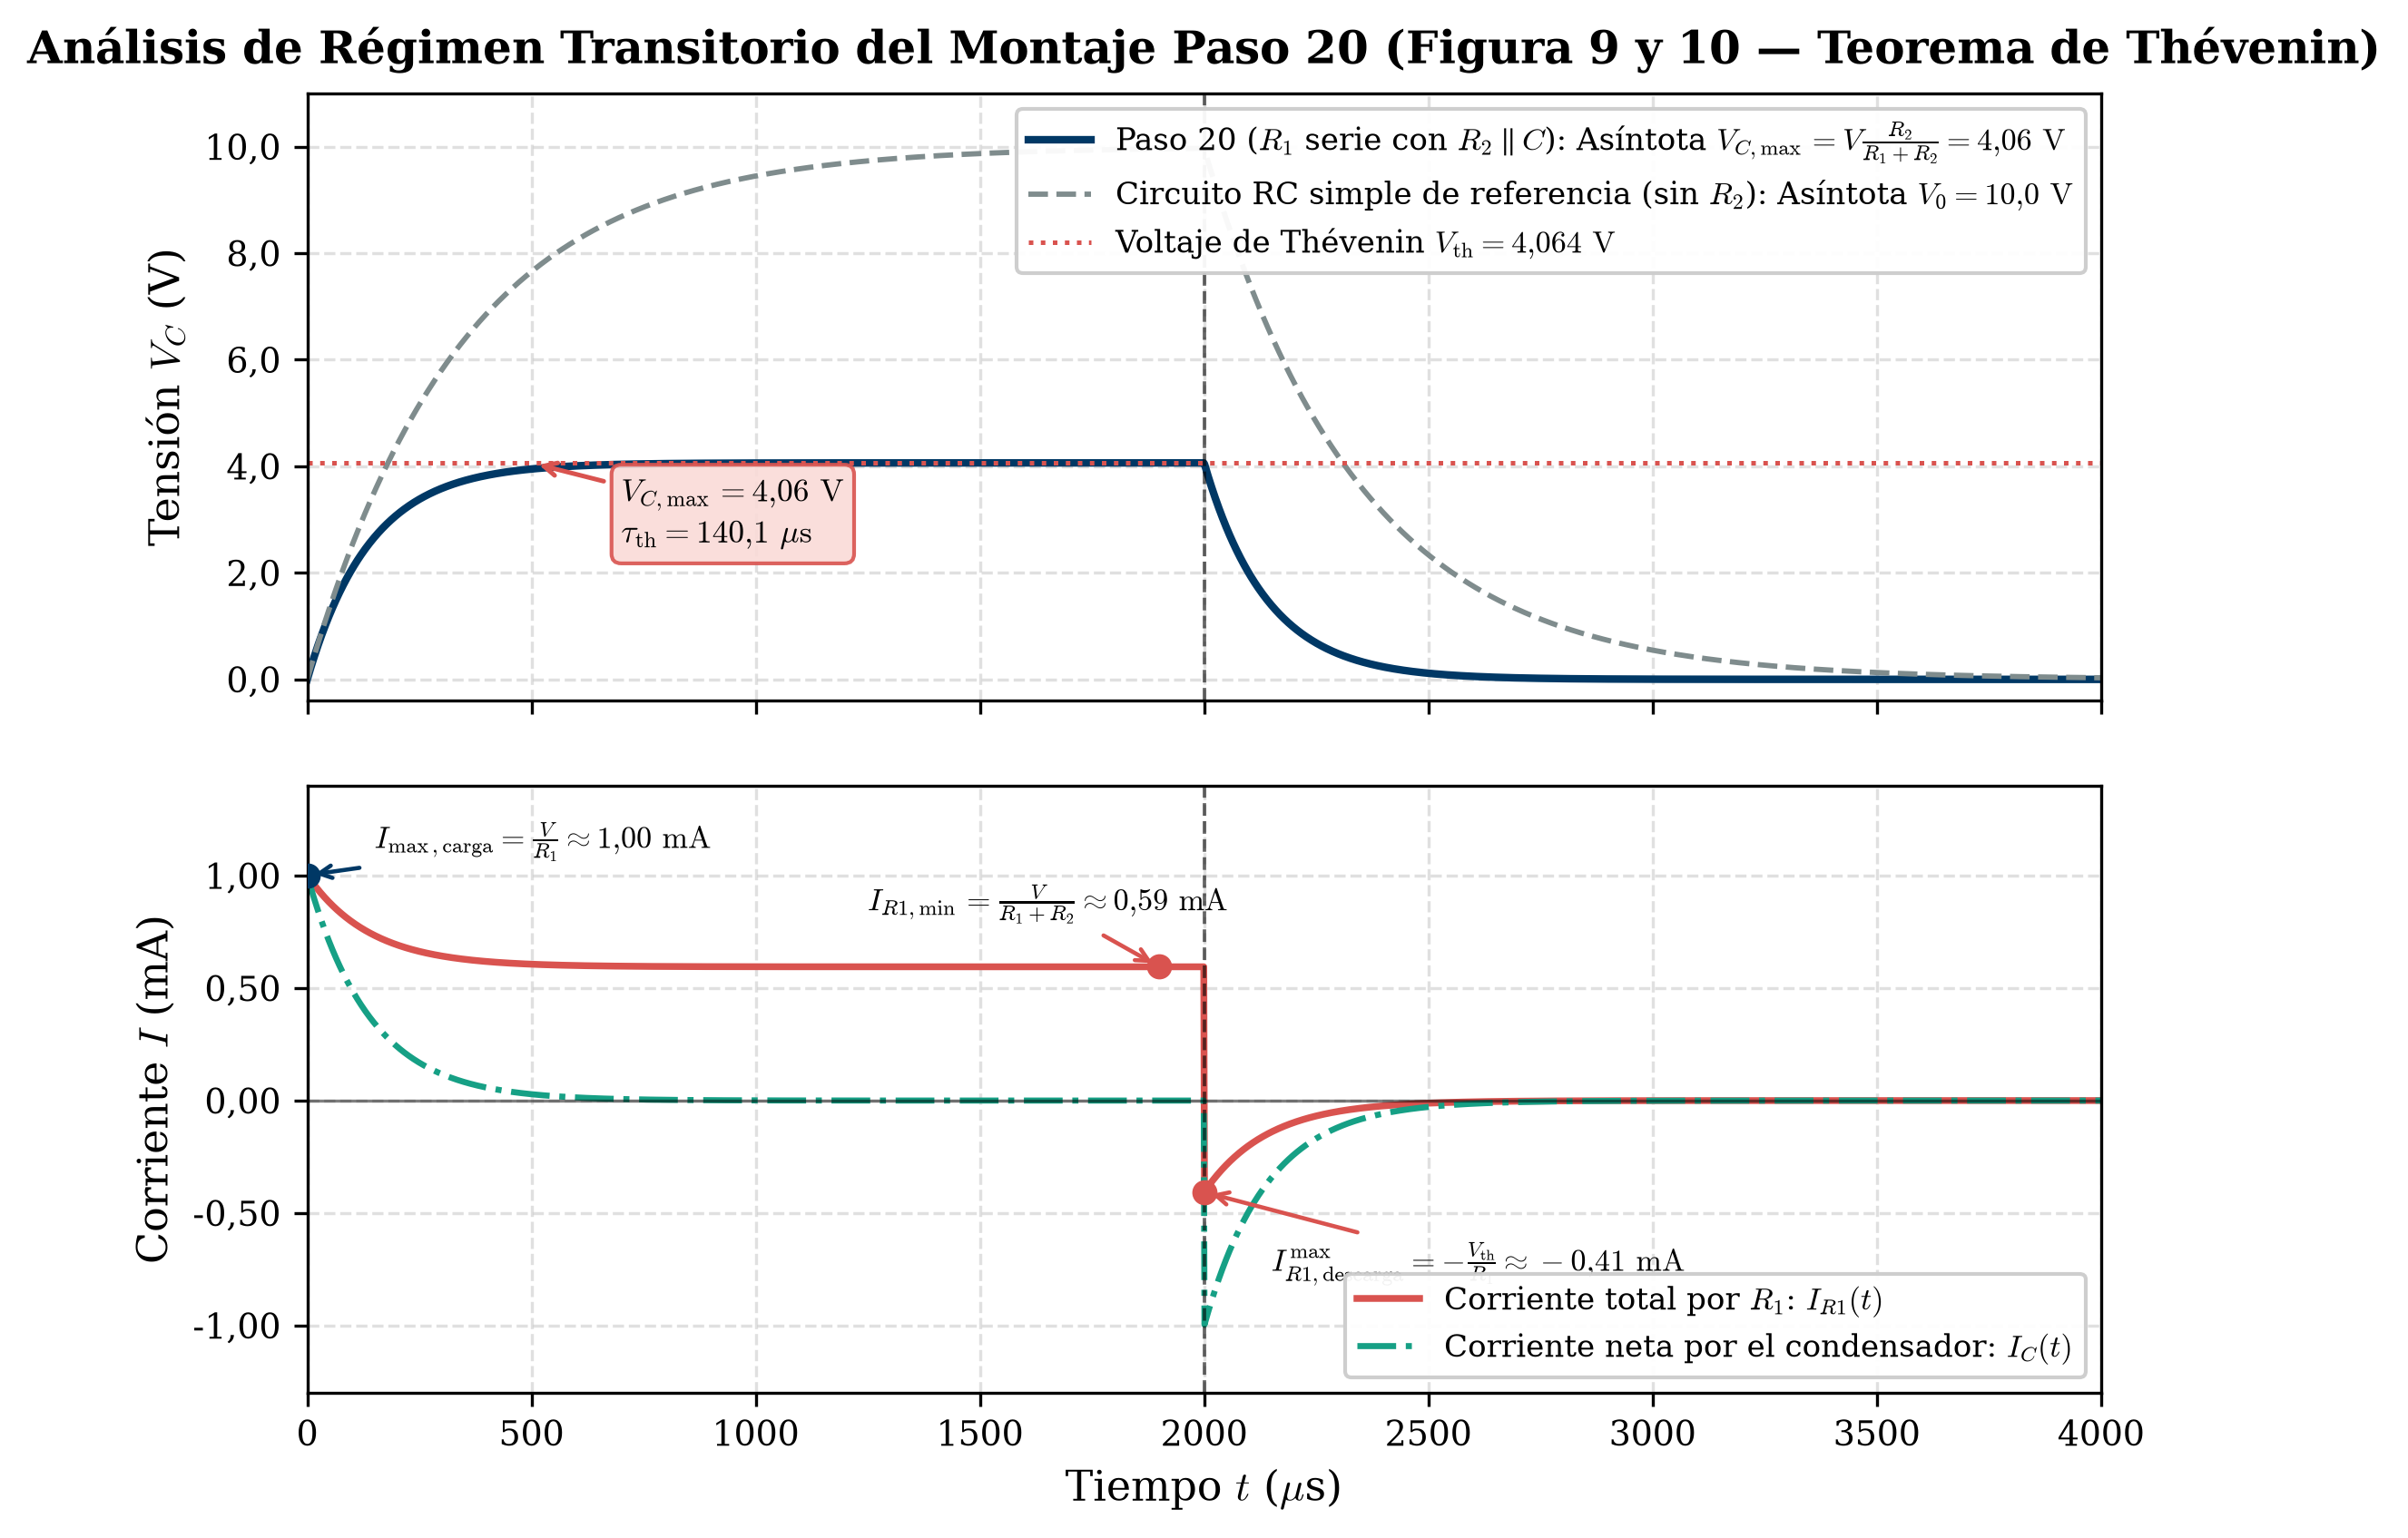
\includegraphics[width=0.88\linewidth]{fig_paso20_thevenin}
    \caption{Respuesta transitoria del circuito mixto correspondiente al paso 20 (Figura 9 y 10 de la guía) con $R_1 = \qty{9,98}{\kilo\ohm}$, $R_2 = \qty{6,832}{\kilo\ohm}$ y $C_3 = \qty{34,55}{\nano\farad}$, analizado mediante el Teorema de Thévenin ($\tau_{\text{th}} = \qty{140,1}{\micro\second}$). Panel superior: tensión $V_C(t)$ alcanzando la asíntota de Thévenin $V_{\text{th}} = \qty{4,06}{\volt}$. Panel inferior: evolución de las corrientes $I_{R1}(t)$ e $I_C(t)$ mostrando las asíntotas no nulas en régimen permanente y el pico de descarga inverso. Figura generada con Python \cite{script_graficas,numpy,matplotlib}.}
    \label{fig:paso20_thevenin}
\end{figure}

Las Figuras~\ref{fig:carga_descarga}, \ref{fig:linealizacion_tau}, \ref{fig:suma_kvl} y \ref{fig:paso20_thevenin} ilustran la concordancia fenomenológica entre el comportamiento experimental y las predicciones teóricas de primer orden. En la siguiente sección (Sección~\ref{sec:analisis_graficas}), se desarrolla la discusión analítica y cuantitativa de estos gráficos, evaluando los coeficientes de correlación $R^2$, la aleatoriedad de los residuos y la prueba de hipótesis del intercepto nulo.
